\section{System Architecture}
The system we have designed consists of multiple parts,
one being a input device, another being a data processer, 
a third one being a communications service and the last one being a presenter.

\subsection{The Input Device}
Our motion tracking device(MTD) has been built in such a fashion that it resembles a wrist watch.
This form factor makes it rather compact.
Additionally alot of people wear watches on a daily basis which makes the device of a recognizable morphology and barely noticeable for people accustomed to such devices.

The MTD contains a list of components, the most important are 6DoF Sensor, Bluetooth and the Arduino microcontroller.

The \textbf{6DoF Sensor} is the heart of the device.
It is a board which contains an accelerometer and a gyroscope.
This means that it is possible to measure movement and rotation of the wrist of anyone wearing the device.
The input received from the 6DoF sensor is the propagated to the \textbf{arduino microcontroller}.
The arduino prepares the raw  values into JSON data. The JSON is then sent using the bluetooth device.

\begin{figure}[!h]
\centering
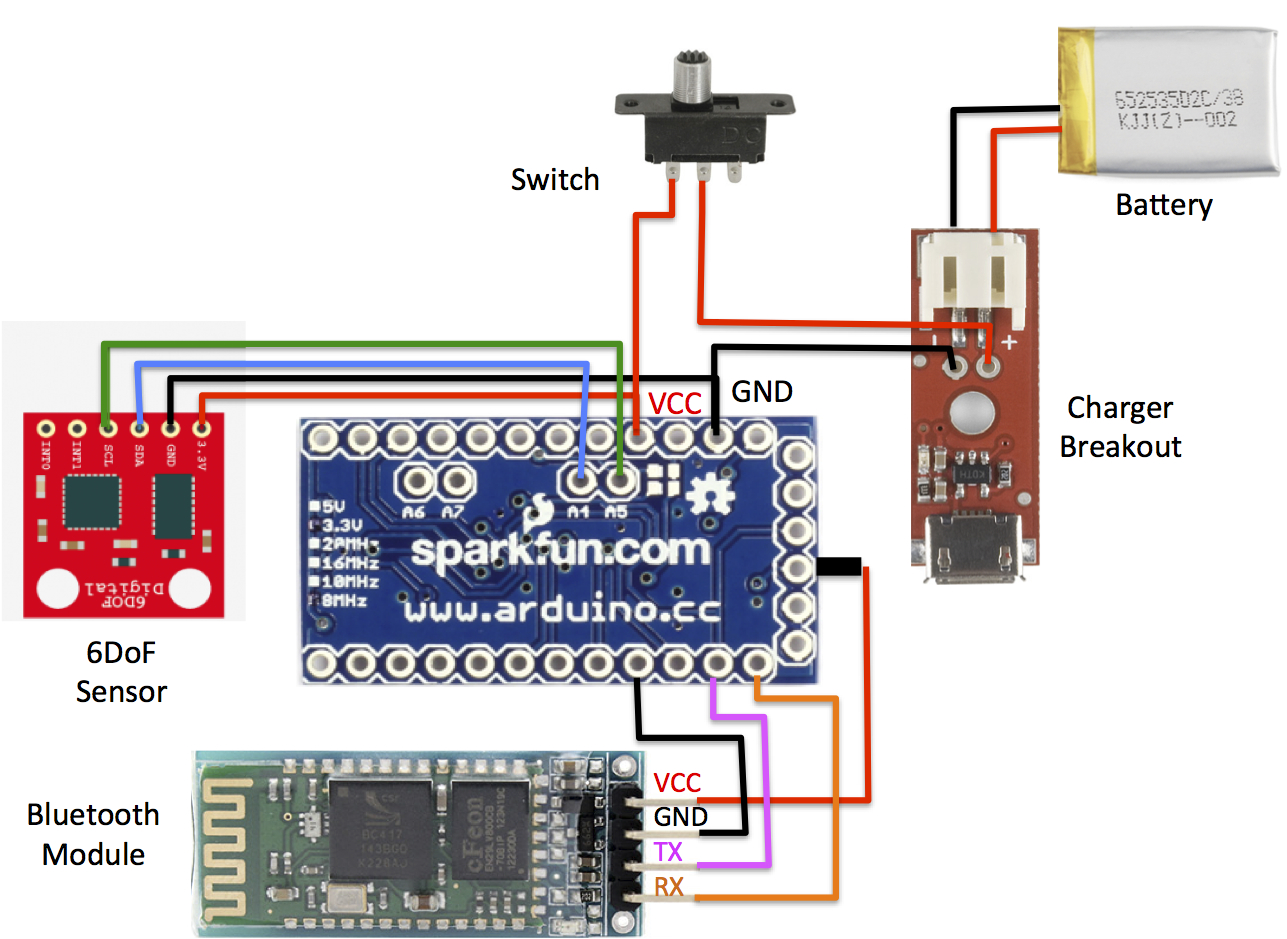
\includegraphics[width=0.9\columnwidth]{img/device_schematic}
\caption{This schematic shows the curcuitry on the device.}
\label{fig:figure1}
\end{figure}

\subsection{Weka Gesture Recognition System}
Since the input device we have built is quite lightweight, data processing needs to be done elsewhere.
This provided us with the challenge of transfering data from one bluetooth capable device to another.
To 

\subsection{Android Application}
The android system is a quite limited system.
It is able to display  an image.
It provides the user with the possibility of panning and zooming a given image.
When the user zooms all the way out panning provides additional functionality.
Pannning left and right will then swap images from the set of loaded images.

\subsection{Webservice}
The communication between the Weka Gesture Recognition System and the Android Application is done by a simple webservice.
It provides GET, POST and DELETE requests which manipulate a queue.

GET pops all the queued gesture recognitions, 
POST pushes a new one to the service and DELETE clears the queue.

\begin{figure}[!h]
\centering
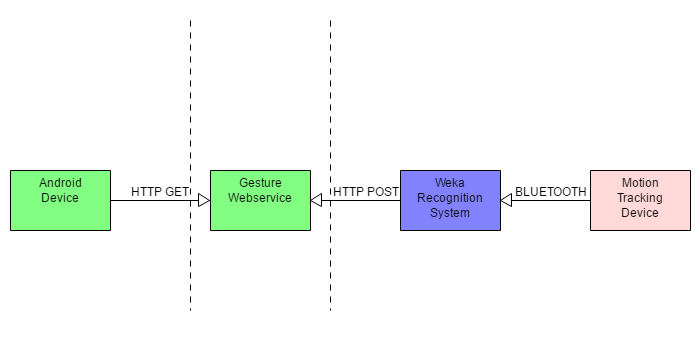
\includegraphics[width=0.9\columnwidth]{img/system_diagram}
\caption{This schematic shows the system interactions.}
\label{fig:figure2}
\end{figure}